% Created 2021-09-11 Sat 16:41
% Intended LaTeX compiler: xelatex
\documentclass[letterpaper]{article}
\usepackage{graphicx}
\usepackage{grffile}
\usepackage{longtable}
\usepackage{wrapfig}
\usepackage{rotating}
\usepackage[normalem]{ulem}
\usepackage{amsmath}
\usepackage{textcomp}
\usepackage{amssymb}
\usepackage{capt-of}
\usepackage{hyperref}
\usepackage[margin=1in]{geometry}
\usepackage{fontspec}
\usepackage{indentfirst}
\setmainfont[ItalicFont = LiberationSans-Italic, BoldFont = LiberationSans-Bold, BoldItalicFont = LiberationSans-BoldItalic]{LiberationSans}
\newfontfamily\NHLight[ItalicFont = LiberationSansNarrow-Italic, BoldFont       = LiberationSansNarrow-Bold, BoldItalicFont = LiberationSansNarrow-BoldItalic]{LiberationSansNarrow}
\newcommand\textrmlf[1]{{\NHLight#1}}
\newcommand\textitlf[1]{{\NHLight\itshape#1}}
\let\textbflf\textrm
\newcommand\textulf[1]{{\NHLight\bfseries#1}}
\newcommand\textuitlf[1]{{\NHLight\bfseries\itshape#1}}
\usepackage{fancyhdr}
\pagestyle{fancy}
\usepackage{titlesec}
\usepackage{titling}
\makeatletter
\lhead{\textbf{\@title}}
\makeatother
\rhead{\textrmlf{Compiled} \today}
\lfoot{\theauthor\ \textbullet \ \textbf{2021-2022}}
\cfoot{}
\rfoot{\textrmlf{Page} \thepage}
\titleformat{\section} {\Large} {\textrmlf{\thesection} {|}} {0.3em} {\textbf}
\titleformat{\subsection} {\large} {\textrmlf{\thesubsection} {|}} {0.2em} {\textbf}
\titleformat{\subsubsection} {\large} {\textrmlf{\thesubsubsection} {|}} {0.1em} {\textbf}
\setlength{\parskip}{0.45em}
\renewcommand\maketitle{}
\author{Houjun Liu}
\date{\today}
\title{Nuclear Physics}
\hypersetup{
 pdfauthor={Houjun Liu},
 pdftitle={Nuclear Physics},
 pdfkeywords={},
 pdfsubject={},
 pdfcreator={Emacs 27.2 (Org mode 9.4.4)}, 
 pdflang={English}}
\begin{document}

\maketitle


\section{Nuclear Physics}
\label{sec:orga0a2e69}
First of all, recall
\href{KBhPHYS201ColoumbsLaw.org}{KBhPHYS201ColoumbsLaw}. Given the
force between two particles is \(\frac{kQ^2}{R^2}\), we could
hand-wavily calculate the \emph{work} between two particles if we know how
much they travel near/far from each other. Through this, we could show
that nuclear forces (through nuclear distance, proton=>electron) are
much larger than that of the chemical forces (atom/atom,
electron=>electron).

\#compilefromnote

Remember: \(A_{nucl} = \frac{1}{10^{10}} A_{atom}\)

\subsection{Radioactivity}
\label{sec:orge369dc6}
Radiation is the emition of waves --- lights, heat, etc. etc. We call
something "radioactive" if it emits ionizing radiation: that it has
enough energy to liberate an electron from an atom.

\subsubsection{Geiger Counter}
\label{sec:org86411dd}
\#inserthowgeigercountersowrk

Because of the fact that Geiger counters require time to discharge,
there is a certain rate called "dead time" during which Geiger counters
simply sit and do nothing. As such, we have to account for this lossy
"deadtime" of Geiger counters by relating the two values with the
following equation

\(T = \frac{M}{1-(M/L)}\), where \(M\) is the measured rate of radiation
and \(L\) is the "dead time" --- the upper limit of the Geiger counter
in question.

\subsubsection{Radio Charge Types}
\label{sec:org2541025}
\begin{itemize}
\item \(\alpha\): positively charged + relatively massive (low
\(\frac{q}{m}\))
\item \(\beta\): negatively charged + relatively high charge (high
\(\frac{q}{m}\))
\item \(\gamma\): neutral
\end{itemize}

This could be seen by how these three types of charge curve into a
magnetic field.

\begin{figure}[htbp]
\centering
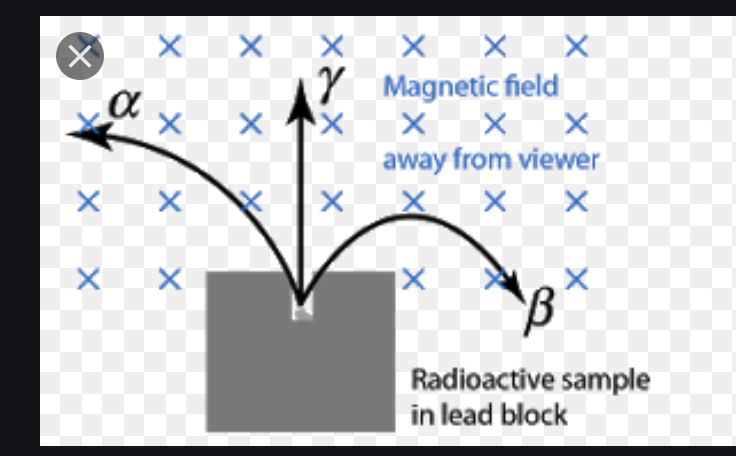
\includegraphics[width=.9\linewidth]{alphabetagamma.png}
\caption{Different charges in a magnetic field}
\end{figure}

Why? Apply right hand rule 1.5.

\subsubsection{Creating a ray}
\label{sec:org5cc2340}
"Split a nucleus, somehow"

\textbf{Alpha Decay}:

\begin{center}
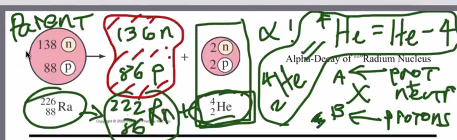
\includegraphics[width=.9\linewidth]{alphadecay.png}
\end{center}

During alpha decay, a massive nucleolus spits out a Helium-resulting
part of itself to get rid of 2 protons and 2 neutrons. So, formally\ldots{}

\begin{center}
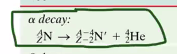
\includegraphics[width=.9\linewidth]{alphadecaybetter.png}
\end{center}

\textbf{Gamma Decay}

Instead of splitting part of the nucleus, gamma decay spits an
electrically excited (so\ldots{} chemistry, charged, energy level, that
stuff) atom into a normal, non-excited atom and also emits a photon.

\begin{center}
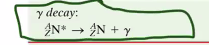
\includegraphics[width=.9\linewidth]{gammadecaybetter.png}
\end{center}

\begin{center}
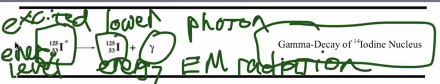
\includegraphics[width=.9\linewidth]{gammadecay.png}
\end{center}

And now, the most confusing one\ldots{}

\textbf{Beta Decay} There's two types of beta decay: "beta-minus" decay and
"beta-plus" decay. When folks talk about just "beta-decay", they are
talking about beta-minus decay.

An element decays from the parent element into a different nucleus.

\emph{Beta minus decay}

\begin{center}
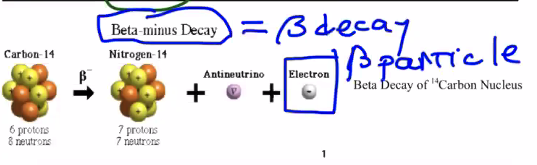
\includegraphics[width=.9\linewidth]{betaminusdecay.png}
\end{center}

In this case, the nucleus gained a proton and lost a neutron.

What happened? A neutron in the nucleus turned into a positive proton
and a negative electron. The newly-formed electron comes flying out as a
"beta-minus" particle. Also, this process creates an "antineutrino",
which is a tiny, charge-less element that will become important later.

\emph{Beta plus decay}

\begin{center}
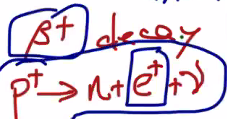
\includegraphics[width=.9\linewidth]{betaplusdecay.png}
\end{center}

This is the opposite of beta-minus decay. The element takes one of its
protons, splits it to a positron (a positive electron, this is
antimatter), a neutrino, and a neutron.

Wait\ldots{} But \emph{how}?

\begin{center}
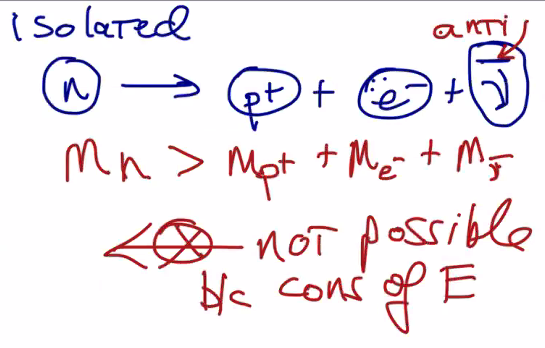
\includegraphics[width=.9\linewidth]{betadecaybackwards.png}
\end{center}

Beta-minus decay makes sense, because it would been energetically
favorable as a neutron is \emph{slightly} more massive and hence will loose
some of the mass during beta-minus decay. But, during beta-plus decay,
the reactants are less massive than the product (!!) --- so thermally it
won't really work out.

\begin{center}
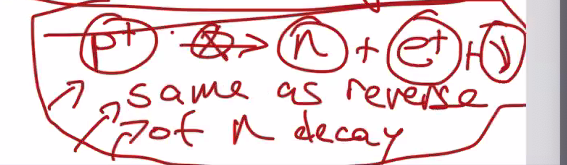
\includegraphics[width=.9\linewidth]{betadecayisreallybackwards.png}
\end{center}

So, in order to actually create beta-plus decay, you have to shove the
protons, antimatter, etc. together really fast with some kinetic energy.
Or, this could happen spontaneously as long as the mass of the daughter
atom is smaller than the mass of the parent (as in\ldots{} as long as mass of
daughter + mass of anti electron + mass of neutrino < mass of parent,
this should work.)

To make sense of this, stop thinking that atoms' masses could be
deducted by just counting the number of neutrons+protons.

\emph{Electron capture}

\begin{center}
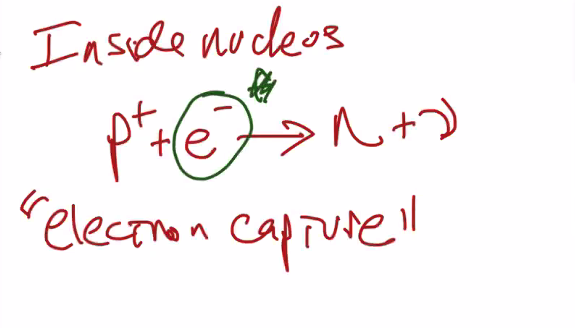
\includegraphics[width=.9\linewidth]{electroncapture.png}
\end{center}

In this case, you will gain one neutron by simply capturing an electron
out of thin air (the electron cloud) and merge it with a proton to form
a neutron and an antineutrino.

So, together\ldots{}

\begin{center}
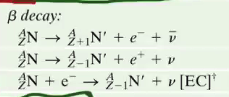
\includegraphics[width=.9\linewidth]{betadecayformal.png}
\end{center}

\emph{Positron Capture}

This basically does not happen; it basically should work in a similar
manner as does electron capture but the opposite.

\begin{center}
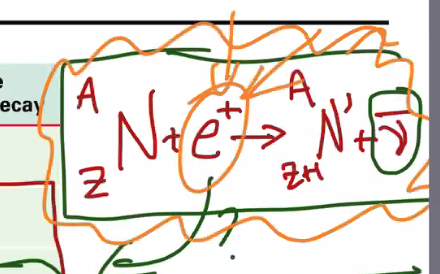
\includegraphics[width=.9\linewidth]{positironcapture.png}
\end{center}

You will need lots of pressure to squish two positive things together
(Electrons + Protons) to fuse.

\subsubsection{Absorbtion of Radioactivity}
\label{sec:org53ed4ec}
\begin{center}
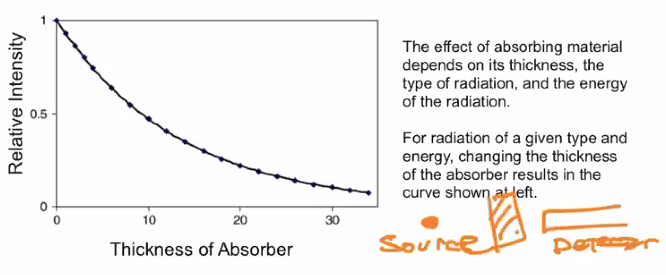
\includegraphics[width=.9\linewidth]{absorbtion.png}
\end{center}

As the thickness of the absorber increases, the relative intensity of
radiation exponentially, asymtotically decreases.

This is similar to the equatino of a dischanging capacitor; namely
\(e^(\frac{-time}{\tau})\)

Instead of a smooth curve, we will decay by 2. We wil use it like a half
life calculation:

\(int = 0.5^{\frac{t}{T}}\), where \(T\) is the thickness required to
absorb 50\%, and \(t\) the thickness of the material. \(int\) should be
the relative intensity of the material --- a percentage (0<=R<=1) that
represents how much of the original, unhindered charge is disturbed.

\begin{center}
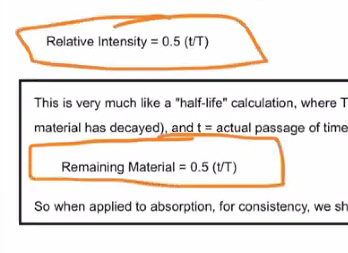
\includegraphics[width=.9\linewidth]{halflife.png}
\end{center}

Relative intensity + half life problem 3:

\begin{center}
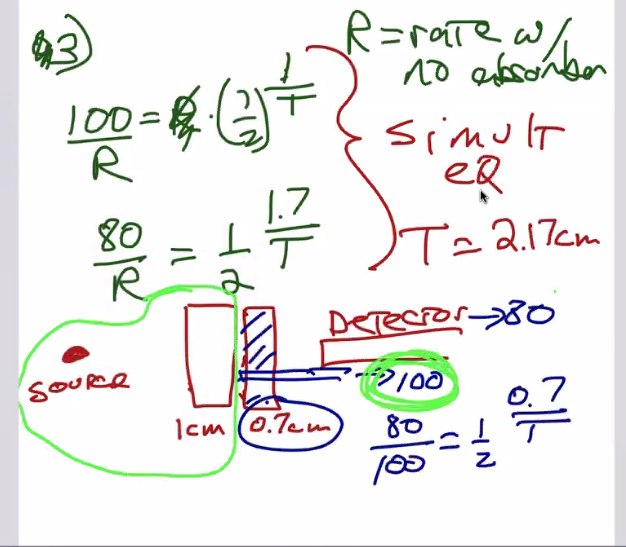
\includegraphics[width=.9\linewidth]{halflifeproctice.png}
\end{center}

\subsubsection{Stopping Rays}
\label{sec:orgcdedba5}
\(\alpha\), \(\beta\), and \(\gamma\) rays are strong in that order ---
alpha rays could be stopped with less insulation than beta than gamma.
HOWEVER, this is given that they all have the same \emph{energy}. Different
rays of the same energy would apply like this, but otherwise the energy
matters especially for betas.

\subsubsection{Atomic Stability}
\label{sec:org01ca3f3}
\textbf{Please remember: most nuclei are stable!! Basically everyday things
does not give you any meaningful amount of radiation.}

\begin{center}
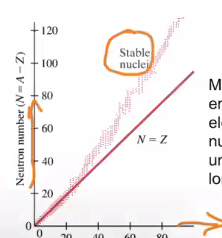
\includegraphics[width=.9\linewidth]{stablenuclei.png}
\end{center}

For relatively low protoned atoms, (\(p < 30\)), stable nuclei is when
\(N \approx p\). For larger atoms, \(N \approx < 1.5P\).

Vocab! Nucleon: neutron + proton.

The standard deviation of \(N\) counts is the \(\sqrt(N)\) if there is a
uniformly random distribution.

\subsection{Fission and Fusion}
\label{sec:orgfaf1feb}
Changes though \textbf{fission} (one nucleaus become two pieces, probably due
to the partent absorbing a neutron, a.k.a. more equal parts of alpha
decay) or \textbf{fusion} (two nuclei joining together to form one)

Due to conservation of energy, not every fission/fusion releases energy.
If fission of A => B C releases energy, fusion of B+C => A wil not.

\begin{figure}[htbp]
\centering
\includegraphics[width=.9\linewidth]{./Pasted image 20210118092740.png}
\caption{Pasted image 20210118092740.png}
\end{figure}

You could think of the energy released as part of fission as the
potential energy of a system.

The bottom row of "mass number" is nucleons w.r.t. the most common
izotope

\begin{figure}[htbp]
\centering
\includegraphics[width=.9\linewidth]{./Pasted image 20210118093104.png}
\caption{Pasted image 20210118093104.png}
\end{figure}

Iron is a terriable way of getting some energy out of a atom because it
has the lowest ever potential energy

Nuclear processes usually end up with Iron; like\ldots{}

\begin{itemize}
\item If you are on the "blue"/"left" region, you release energy by
fusioning into iron (add stuff up until you get to stable iron.)
\item If you are on the "yellow"/"right" region, you release energy by
fissioning into iron (split until you get to iron)
\end{itemize}

\noindent\rule{\textwidth}{0.5pt}

But actually this is kind of a lie. It is actully a contour of all
different izotopes, measured in "binding" energy and not PE. The
\textbf{binding energy} is how forcibly the nucleaus are bound together --- the
more tighly bound, the more energy it would require to break the
binding.

Also, Binding Energy is measured in MeV, which convents to Joules with
\(1 MeV = 1.6 \times 10^{-13} J\).

Nuclear fission is triggered by smushing a neutron into an atom.

For instance\ldots{}

\href{Pasted image 20210118094127.png.org}{Pasted image
20210118094127.png}

\section{Data Shape}
\label{sec:org004b901}
\begin{center}
\begin{tabular}{llll}
Thickness & Count Rates & Count Time & Result: Normalized Count Rate\\
\hline
\end{tabular}
\end{center}

This will, of course, result in a graph of thickness vs. count rate.

Goal: finding the best T and the +/- range that would fit the rates

\href{Pasted image 20210120111507.png.org}{Pasted image
20210120111507.png}

\subsection{What is "best fit"}
\label{sec:orgc298695}
\href{Pasted image 20210120112247.png.org}{Pasted image
20210120112247.png}

When data is uncertain, best fit should minimize
\(\sum \frac{D_i-M_i}{\sigma_i}^2\). Think as "how many standard
deviations away" is the uncertainty. This is also called "pearson's
statistic"

With this piece of information, at different discrete values of T, we
could have a graph of T vs. S. At the minimum of that curve, that's the
best fit!

Smin should be about \# of datapoints - \# of parametres

If Smin << \# dp - \# params, you did something wrong.

If Smin >> \# dp - \# params, sigma were probably underestimated/not the
only sources of error

\section{Lab}
\label{sec:org845fdcf}
\begin{enumerate}
\item Apply deadtime correction to both rate and unceartainty in the rate
\item Subtract (background, \emph{no need to correct deadtime here}, propergate
error)
\item Divide measured rates by the rate with no absorber to figure the
relative rates. Propergate error. This should be 1ish
\item 
\end{enumerate}

\noindent\rule{\textwidth}{0.5pt}

2 types of nuclear energy generator

\begin{enumerate}
\item Pressurized water reactor => Pressured, superheated water superheats
nearby water to steam
\item Boiling water reactor => Reactor directly heat
\end{enumerate}

Pressured water reactor has control SCRAM rods above, because steam is
not dried within the reactor. Boiling water reactors have control rods
below, because the output steam's dryer is above and hence control rods
needs to be place below.

The fuel rods contain UO2,with about 3\% being U. The rest is the
radioactive slowly decaying common 238U. Uranium ore comes out as 0.7\%
235U, but we need that to be 3\% b/c fissioning 238U is not helpful, so a
process called "enrichment" helps purify the Uranium and rid of 238 to
leave only 235.

Raw fuel isn't super radioactive. But, once the fuel is insterted, a
neutron gets shot in and the recator starts. Control rods could be
inserted in to stop teh reaction. \#why

Spent fuel is radioactive. Raw U238 does not go through much decay
(see\ldots{} 4.8 Billion Years), but what comes out of the fissioning process
is two random elements that could be quite radioactive.

Also, Plutonium, a result of Uranium fission, also is toxic chemically
and emits alpha rays. This could be used as a nuclear weapon in the
"emits alpha rays" sense but also used as a slightly more inefficient
way of creating lots of heat. Hence, this is fiercely protected.

After fission stops, 5-10 megawatts still gets generated. This, if not
cooled by 8g/s of water, will result in zicalloy interaction and
hydrogas formation due to chemistry. And that will brow up (and the
thing that blows up includes plutonium!).

The radiation from spent fuel glows blue, because it travels faster than
light travels in water so specific rays comes out

In order for the radiation to decay down into standard radiation, one
would need to store 10,000+ years for 10\% original radiation. However,
reprocessving techniques could lower that to around 200 years

Nuclear Radiation ionizez atoms and molecules, which mess things up
chemically

\noindent\rule{\textwidth}{0.5pt}

1 Bq per second means that the source disintgrates once per seciond. 1
currie means that the source disntergrates at 3.7 * 10\textsuperscript{10} bq

1rad: a material absorbed 0.01 J per kg of absorbing material.

Effective dose (rem) = rad * QF (quality factor). For most cases,
quality factor is 1 for most common radiation. For neutrons and alpha
particles, it is 3 and up to 20 respectively, but the former could only
be seen in the middle of a recator or if a bomb just went off and the
latter could be block by some sheets of clothing

Rad/Rem/Siverts => Measure of \emph{absorbtion of energy} per kilogram over
time Bq/Currie => Measure of Emission and source strength

Bottom line: don't worry about the siverts you recieve\ldots{} unless you eat
a radioactive source, because then its emitting in you

Radiation absorbtion results

\begin{center}
\begin{tabular}{ll}
Severts number & Effect\\
\hline
0.5 Sv immediately & 4\% chance of cancer during lifetime, no immediate effect\\
1-5 Sv immediately & 50\% chance of death\\
6+ Sv immediatlely & Bye bye birdy, 30 days\\
\end{tabular}
\end{center}

Note: food sterialized by radioactivity is not radioactive\ldots{}
\end{document}
